\documentclass{standalone}
\usepackage{tikz}
\usetikzlibrary{positioning}
\usetikzlibrary{mindmap,trees}
\usepackage{verbatim}

\begin{document}
\pagestyle{empty}
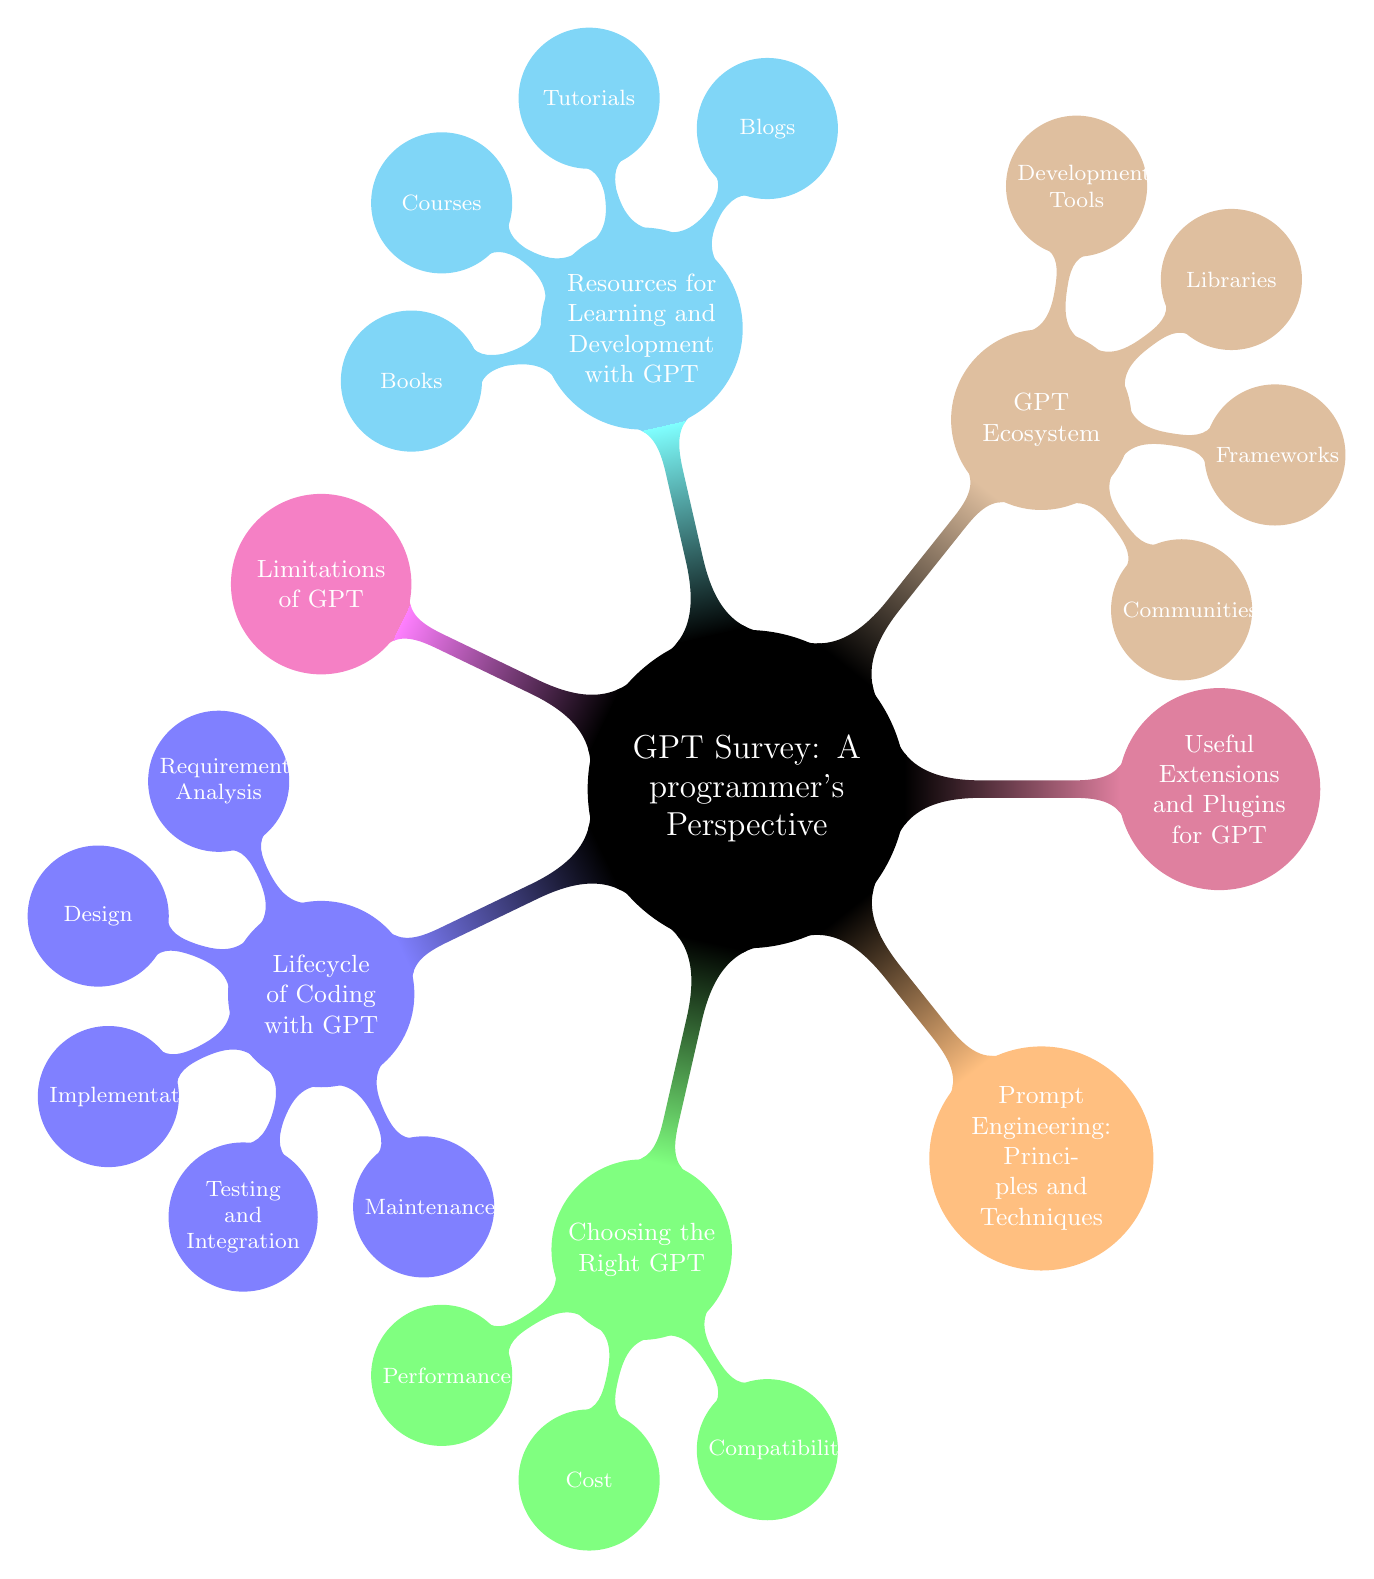
\begin{tikzpicture}[mindmap, grow cyclic, every node/.style=concept, concept color=black, text=white,
  level 1/.append style={level distance=6cm, sibling angle=360/\the\tikznumberofchildren},
  level 2/.append style={level distance=3cm, sibling angle=45},
]

  \node {GPT Survey: A programmer's Perspective}
    child[concept color=blue!50] { node {Lifecycle of Coding with GPT}
      child foreach \y in {
        {Requirement Analysis},{Design},{Implementation},{Testing and Integration},{Maintenance}
      } {
        node[concept] {\y}
      }
    }
    child[concept color=green!50] { node {Choosing the Right GPT}
      child { node {Performance}}
      child { node {Cost}}
      child { node {Compatibility}}
    }
    child[concept color=orange!50] { node {Prompt Engineering: Principles and Techniques}}
    child[concept color=purple!50] {node {Useful Extensions and Plugins for GPT}}
    child[concept color=brown!50] { node {GPT Ecosystem}
      [clockwise from=30]
      child {node[concept] {Development Tools}}
      child {node[concept] {Libraries}}
      child {node[concept] {Frameworks}}
      child {node[concept] {Communities}}
    }
    child[concept color=cyan!50] {
        node[concept] (n) {Resources for Learning and Development with GPT}
        [clockwise from=90]
        child{node[concept]{Books}}
        child{node[concept]{Courses}}
        child{node[concept]{Tutorials}}
        child{node[concept]{Blogs}}
    }
    child[concept color=magenta!50] {
        node[concept](o){Limitations of GPT}
    };
\end{tikzpicture}
\end{document}